\section{Kravspecificering og Use cases}
I dette afsnit vil vi beskrive vores kravspecificering og vores Use cases, som vi har udarbejdet til denne rapport.
\subsection{Kravspecificering}
\todo[inline]{Thomas M: Indsætte de få tvivlskrav, der er i dropbox}
I dette afsnit har vi taget udgangspunkt i kundens vision. Vi har læst den igennen, og stillet spørgsmålstegn, ved de ting, der kunne væere tvivl om.
\begin{enumerate}
\item Spillerne slår på skift med 2 terninger, men vi ved ikke hvem starter?
\item Hvert felt har positiv eller negativ effekt på spillerens pengebeholdning, men hvorfor er felt syv hverken eller?
\item Spillerne starter med en beholdning på 1000, men er det kr, rubler, eller andet(Skal vi forberede til komma tal)?
\item Spillet slutter når en spiller har 3000, men kan man komme over, og så prøve at ramme negative felter?
\item Spillet skal let kunne oversættes, men er der et foretrukkent sprog at oversættes fra (Er det kode eller tale)?
\item Det skal være let at skifte terninger, men skal det testes?
\item Spilleren og pengebeholdningen skal kunne bruges i andre spil, men i hvilken forstand?
\item Hvad skal der ske hvis en spiller ville have fået en negativ balance på kontoen pga. negative konsekvenser?
\end{enumerate}
Vores kontakt i firmaet, som er vores projektleder, har besvaret disse punkter på følgende måde
\begin{enumerate}
\item Vi må selv om det, men kunden anbefaler den nemmeste/billigste løsning
\item Skal ikke laves om. Det er med vilje feltet ikke har negativ eller positiv konsekvens.
\item Kunden ønsker ingen brug af kommatal (Heller ikke senere). Hvis vi vælger at oversætte skal vi kunne oversætte valuta. Derfor ønskes en unavngiven valuta.
\item Så snart det ønskede beløb eller mere er opnået slutter spillet. Hvis en spiller kommer under nul, har han tabt spillet.
\item Der er ikke noget foretrukkent sprog. Vi skal bare hoilde os til samme sprog hele vejen igennem. Der er ikke tale om andre kodesprog.
\item Vi skal ikke dokumenteres med test, om man kan skifte terninger, men det forventes at virke.
\item Det bliver måske en anden form for terningespil, så vi skal ikke forberede klasserne til noget ekstraordinært, som ikke er relevant.
\item Hvis en spiller kommer under nul, har han tabt spillet.
\end{enumerate}
\subsection{Use Cases}
\todo[inline]{Thomas A: Indsæt tekst fra fully dresses og brief + diagram}
Vi vil i dette afsnit beskæftige os med 2 use cases, som er beskrevet i nedenstående diagram. Til vores spil har vi lavet en fully dressed use case, og til vores test har vi blot lavet en brief use case.
\subsubsection{Use Case Diagram}
\begin{figure}[ht]
\centering
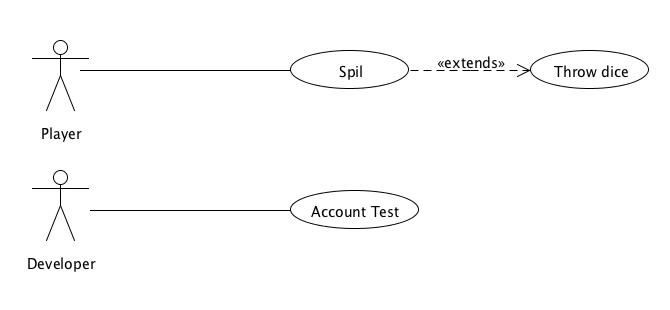
\includegraphics[scale=0.5]{UseCaseDiagram.jpg}
\caption[<Text for the list of figures>]{Use Case Diagram}
\label{fig:figure 2}
\end{figure}
\newpage
\subsubsection{Fully Dressed Use Case}
Vi har i dette afsnit beskrevet vores use case med en fully dressed use case for spil.
\subsubsection*{Use Case}
Spil
\subsubsection*{Scope}
Terningspil
\subsubsection*{Level}
User Goal
\subsubsection*{Primary actor}
Spiller
\subsubsection*{Stakeholders and Interests}
Spiller: vil vinde spillet
\subsubsection*{Preconditions}
Eclipse er installeret på maskinen.
\\
Programmet er startet.
\subsubsection*{Main Success Scenarie:}
\begin{enumerate}
\item Spiller starter spillet
\item Spiller indtaster Navn
\item Spiller Ruller med terningerne
\item Spiller lander på et felt med positiv konsekvens
\item Spiller modtager point
-- Spiller gentager punkt 3-5 indtil 3000 eller mere er opnået
\item System checker vinder
\item System viser vinder
\item System lukker ned
\end{enumerate}
\subsubsection*{Extensions Alternative scenarier:}
*a - til hvert et tidspunkt
\begin{enumerate}
\item Spiller lukker spillet ved at taste "q"
\end{enumerate}
4a. Spiller lander på et felt med negativ konsvens
\begin{enumerate}
\item Spiller får trukket point
\item Spiller ryger under 0 point
-- punkt 6-8 i main success aktiveres
\end{enumerate}
4b. Spiller lander på et felt uden konsekvens
\begin{enumerate}
\item Spiller for trukket point
\item a Spiller ryger under 0 point
-- punkt 6-8 i main success aktiveres
\item b Spiller rammer felt 10. uden at komme under 0, hviket giver ekstra tur. 
-- punkt 3 i main success aktiveres
\end{enumerate}
\subsubsection*{Specielle Krav:}
\begin{itemize}
\item Skal kunne køre på en Windows maskine med Java EE på DTU's computere
\item Skal kunne spilles af en almindelig bruger
\end{itemize}
\subsubsection{Brief Use Case Account test}
Vi har valgt at lave en brief use case over vores test.
\\

\textbf{Account Test}
En udvikler tester klassen med forskellige grænse og middelværdier, der er foruddefineret i klassen. Resultaterne printes ud i konsollen, og udvikleren ser om resultaterne fra testen, stemmer overens med de forventede resultater.